\documentclass[12pt]{article}

%%%%%%%%%%%%%%%%%%%%%%%%%%%%%%%%%%%%%%%%%%%%%%%%%%%%%%%%%%%%%%%%%%%%%%%%%%%%%%%%%%%%%%%%%%%%%%%%%%%%%%%%%%%%%%%%%%%%%%%%%%%%%%%%%%%%%%%%%%%%%%%%%%%%%%%%%%%%%%%%%%%%%%%%%%%%%%%%%%%%%%%%%%%%%%%%%%%%%%%%%%%%%%%%%%%%%%%%%%%%%%%%%%%%%%%%%%%%%%%%%%%%%%%%%%%%

\usepackage[onehalfspacing]{setspace}
\usepackage{graphicx}
\usepackage{epstopdf}
\usepackage{blindtext}
\usepackage{adjustbox}
\usepackage{natbib}
\usepackage{lipsum}

\usepackage[paperwidth=210mm,paperheight=297mm,left=27mm,right=27mm,top=27mm,bottom=27mm]{geometry}

\usepackage{bibentry}

\bibliographystyle{apalike}

\title{2020 STATA ECONOMETRICS WINTER SCHOOL\thanks{January 21-25, 2019 -- Faculdade de Economia da Universidade do Porto, Portugal}}
\date{2020\\ January}
\author{Anabela Carneiro\\ U Porto
\and João Cerejeira \\ U Minho
\and Miguel Portela \\ U Minho
\and Paulo Guimarães \\ Banco de Portugal \& U Porto}

\begin{document}

\maketitle

\section{Introduction}\label{sec:intro}

\lipsum

\section{Literature}

\lipsum

\section{Empirical analysis}

\subsection{Data}

\lipsum

Figure \ref{fig:incdensity} sets the stage for our example, while Table \ref{tb:descriptives} shows descriptive statistics for the data used in the regression analysis. It shows a kerndel density for income. Table \ref{tb:regresults} presents our regressions. One could follow the book by \cite{acemoglu2016} to motivate the discussion. A thorough discussion of Econometrics is provided by \cite{greene2017} (see also \citet{verbeek2012}).\footnote{\cite{wooldridge2015introductory} makes a good introduction to Econometrics.} We can also see \cite{harmon2003returns} or \cite{robeyns2003sen} ...

\begin{table}[h]\caption{Descriptive statistics}\label{tb:descriptives}
\begin{center}
\resizebox{0.9\textwidth}{!}
	{\begin{tabular}{lcccccc} \hline
VARIABLES & N & mean & p99 & sd & min & max \\ \hline
 &  &  &  &  &  &  \\
Real GDP per worker & 857.000 & 19,901.781 & 74,706.383 & 21,470.140 & 396.761 & 271,192.125 \\
Education (in years) & 857.000 & 4.769 & 11.430 & 2.882 & 0.040 & 12.250 \\
Capital & 234.000 & 5.498e+11 & 1.021e+13 & 1.582e+12 & 1.195e+09 & 1.121e+13 \\
Degree of openness & 857.000 & 62.857 & 290.202 & 52.178 & 2.320 & 395.977 \\
 &  &  &  &  &  &  \\ \hline
\end{tabular}}
\end{center}
\end{table}


\begin{table}\caption{Descriptive statistics by country -- logout}
\centering
\resizebox{0.85\width}{!}{%
\begin{tabular}{lccccccccc} \hline
Country & mean & sd & min & p5 & p50 & p90 & p99 &  &  \\ \hline
Afghanistan & 0.928 & 0.159 & 0.730 & 0.730 & 0.910 & 1.140 & 1.140 &  &  \\
Algeria & 1.975 & 1.438 & 0.650 & 0.650 & 1.315 & 4.315 & 4.720 &  &  \\
Argentina & 6.403 & 1.395 & 4.360 & 4.360 & 6.250 & 8.305 & 8.490 &  &  \\
Australia & 9.968 & 0.401 & 9.300 & 9.300 & 10.06 & 10.57 & 10.57 &  &  \\
Austria & 7.732 & 0.844 & 6.710 & 6.710 & 8.220 & 8.800 & 8.800 &  &  \\
Bahrain & 3.387 & 1.795 & 1.370 & 1.370 & 3.120 & 6.090 & 6.090 &  &  \\
Bangladesh & 1.572 & 0.685 & 0.790 & 0.790 & 1.680 & 2.450 & 2.450 &  &  \\
Barbados & 7.653 & 1.546 & 5.220 & 5.220 & 8.190 & 9.110 & 9.110 &  &  \\
Belgium & 8.126 & 0.433 & 7.460 & 7.460 & 8.160 & 8.730 & 8.730 &  &  \\ \hline
\end{tabular}
}
\end{table}


\begin{table}[ht]\caption{Descriptive statistics by year -- tabout}
\centering
\resizebox{0.85\width}{!}{%
    \begin{tabular}{l|c|ccccc|cc}
\hline
	& & \multicolumn{5}{c}{Means} & \multicolumn{2}{|c}{Medians} \\ \hline
& Obs. & Pop. & OpenK & GDP & Education & ln GDP & ln Capital & $\Delta_{GDP}$ \\
\hline
Year&&&&&&&& \\
1950&16&27,877.8&35.5&10,744.6&3.4&9.1\%&& \\
1955&2&13,162.5&49.0&9,727.7&5.0&8.8\%&&0.28\% \\
1960&78&21,242.5&49.5&11,999.7&3.6&8.9\%&&0.24\% \\
1965&79&23,208.5&51.2&14,346.9&3.6&9.1\%&&0.18\% \\
1970&95&22,366.0&58.4&18,371.2&3.9&9.2\%&24.7&0.16\% \\
1975&96&34,289.6&59.0&18,179.0&4.1&9.3\%&25.0&0.11\% \\
1980&97&36,974.5&64.6&23,061.3&4.7&9.4\%&25.3&0.12\% \\
1985&96&40,684.6&61.6&20,407.0&5.0&9.4\%&25.2&0.01\% \\
1990&101&42,267.4&66.5&21,947.4&5.5&9.4\%&25.5&0.06\% \\
1995&99&46,936.5&73.8&23,535.4&5.9&9.4\%&&0.03\% \\
2000&98&50,089.0&80.4&26,142.1&6.3&9.5\%&&0.07\% \\
\hline
Total&857&35,818.0&62.9&19,901.8&4.8&9.3\%&25.2&0.09\% \\

\hline
\end{tabular}
}
\end{table}


\begin{figure}[ht]
	\begin{center}
		\includegraphics[scale = 0.3,trim = 0.0 0.0 0.0 0.0,clip]{income_density.png}
		\caption{Income density}\label{fig:incdensity}
	\end{center}
\end{figure}

\begin{figure}[ht]
	\begin{center}
		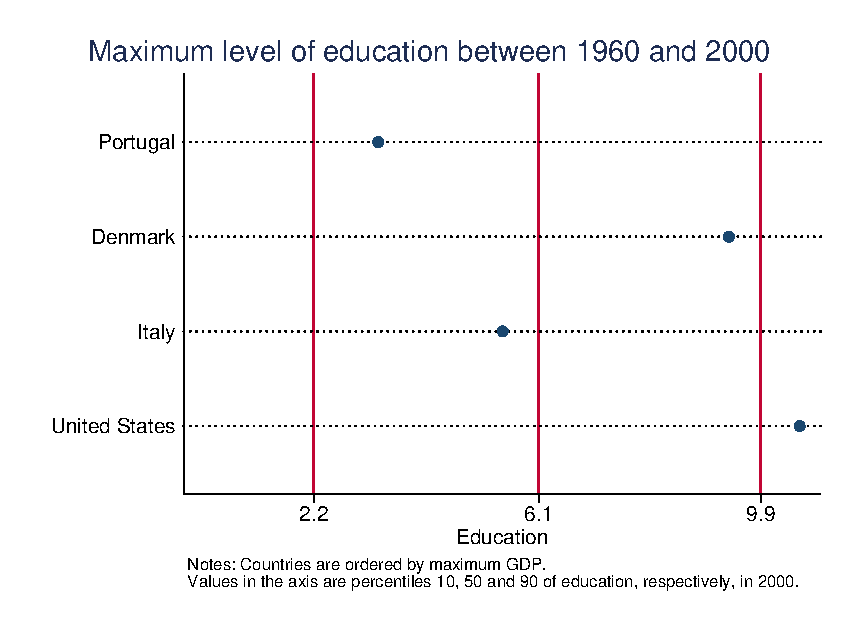
\includegraphics[scale = 0.8,trim = 0.0 0.0 0.0 0.0,clip]{example1.eps}
		\caption{Level of education}\label{fig:education}
	\end{center}
\end{figure}

\lipsum

\subsection{Models \& regressions}

\lipsum

\begin{table}[ht]
\caption{Regression analysis -- using esttab}\label{tb:regresultsb}
	\begin{center}
		{
\def\sym#1{\ifmmode^{#1}\else\(^{#1}\)\fi}
\begin{tabular}{l*{6}{c}}
\hline\hline
            &\multicolumn{1}{c}{OLS (1)}&\multicolumn{1}{c}{OLS (2)}&\multicolumn{1}{c}{OLS (3)}&\multicolumn{1}{c}{FE}&\multicolumn{1}{c}{BE}&\multicolumn{1}{c}{RE}\\
\hline
Average education&       0.317\sym{***}&       0.212\sym{***}&       0.214\sym{***}&      -0.011         &       0.209\sym{***}&       0.064\sym{***}\\
            &     (0.009)         &     (0.020)         &     (0.019)         &     (0.029)         &     (0.044)         &     (0.025)         \\
[1em]
Log capital &                     &       0.125\sym{***}&       0.198\sym{***}&       0.222\sym{***}&       0.229\sym{***}&       0.207\sym{***}\\
            &                     &     (0.029)         &     (0.031)         &     (0.036)         &     (0.071)         &     (0.033)         \\
[1em]
Openness    &                     &                     &       0.006\sym{***}&      -0.002\sym{***}&       0.009\sym{***}&      -0.002\sym{***}\\
            &                     &                     &     (0.001)         &     (0.001)         &     (0.003)         &     (0.001)         \\
\hline
\(N\)       &         857         &         234         &         234         &         234         &         234         &         234         \\
R$^2$       &        0.58         &        0.54         &        0.59         &        0.48         &        0.63         &                     \\
RMSE        &        0.78         &        0.70         &        0.67         &        0.14         &        0.65         &        0.15         \\
\hline\hline
\multicolumn{7}{l}{\footnotesize Notes: standard errors in parenthesis. Significance levels: *, 10\%; **, 5\%; ***, 1\%.}\\
\multicolumn{7}{l}{\footnotesize The dependent variable is ln real GDP per worker. All models include a constant.}\\
\multicolumn{7}{l}{\footnotesize Models OLS (3) till RE include time dummies.}\\
\multicolumn{7}{l}{\footnotesize Source: own computations.}\\
\end{tabular}
}

	\end{center}
\end{table}

\begin{table}[ht]
\caption{Regression analysis -- using outreg}\label{tb:regresults}
	\begin{center}
		\input{growth_analysis_frag}
	\end{center}
\end{table}

\section{Final remarks}

\lipsum


\bibliography{references}

\end{document}
